\chapter{Specyfikacja wewnętrzna}
\label{ch:05}

% % % % % % % % % % % % % % % % % % % % % % % % % % % % % % % % % % % 
% Pakiet minted wymaga importu: \usepackage{minted}                 %
% i specjalnego kompilowania:                                       %
% pdflatex -shell-escape main                                       %
% % % % % % % % % % % % % % % % % % % % % % % % % % % % % % % % % % % 
W niniejszym rozdziale Specyfikacji Wewnętrznej dokładnie omówione zostaną kluczowe elementy związane z implementacją projektu. Zaprezentowana będzie architektura systemu, opisane zostaną użyte biblioteki i moduły, przedstawione zastosowane algorytmy, a także zamieszczone zostaną diagramy sekwencyjne, fragmenty kodu oraz idea, która kierowała procesem tworzenia aplikacji. Celem tego rozdziału jest szczegółowe przybliżenie struktury wewnętrznej projektu, zrozumienie jego komponentów oraz logiki działania.

%\section{\textbf{Przedstawienie idei}}
%
%Aplikacja Infektosym jest narzędziem symulacyjnym, które zostało stworzone z myślą o zrozumieniu i analizie rozprzestrzeniania się zarażeń w przestrzeni biurowej. Głównym celem projektu jest dostarczenie interaktywnej platformy umożliwiającej obserwację, analizę oraz testowanie scenariuszy związanych z potencjalnymi wirusowymi infekcjami w środowisku pracy.
%
%\begin{itemize}
%	\item \textbf{Cele Projektu:}
%	\begin{itemize}
%		\item Zapewnienie realistycznego modelu symulacji, uwzględniającego codzienne zachowania ludzkie w biurze.
%		\item Możliwość dostosowywania parametrów symulacji, takich jak dystans zarażenia, czas do zarażenia czy skuteczność maseczek.
%		\item Wizualizacja procesu rozprzestrzeniania się patogenów w czasie rzeczywistym.
%	\end{itemize}
%	\item \textbf{Koncepcje i Założenia:}
%	\begin{itemize}
%		\item Implementacja agentowego podejścia, gdzie każdy osobnik w symulacji podejmuje indywidualne decyzje i reaguje na otoczenie.
%		\item Duża parametryzacja symulacji, umożliwiająca dostosowanie scenariuszy do różnych warunków i kontekstów.
%	\end{itemize}
%	\item \textbf{Kierunki Rozwoju:}
%	\begin{itemize}
%		\item Wprowadzenie zaawansowanych funkcji interakcji między agentami, uwzględniających bardziej złożone scenariusze zachowań.
%		\item Integracja z danymi epidemiologicznymi dla bardziej precyzyjnych analiz i prognoz.
%		\item Dalsza optymalizacja interfejsu użytkownika i dostępność na różnych platformach.
%		\item Wprowadzenie innych scenariuszy np. Szpital, Osiedle, Centrum Handlowe.
%	\end{itemize}
%\end{itemize}

\section{\textbf{Architektura systemu}}

Architektura systemu aplikacji opiera się na modularnym podejściu, skupiającym się na kilku kluczowych skryptach odpowiedzialnych za różne aspekty symulacji.

\begin{itemize}
	\item \textbf{InterfaceScript:}
	\begin{itemize}
		\item Odpowiada za interakcję z użytkownikiem, umożliwiając mu dostosowywanie parametrów symulacji za pomocą sliderów.
		\item Obsługuje przyciski kontroli, takie jak start, pauza, restart, co zapewnia płynną kontrolę nad symulacją.
		\item Wyświetla istotne statystyki dotyczące aktualnego stanu symulacji, umożliwiając użytkownikowi bieżącą analizę danych.
	\end{itemize}
	
	\item \textbf{GlobalClockScript:}
	\begin{itemize}
		\item Pełni rolę zegara w aplikacji, monitorując czas zarówno w skali symulacji, jak i rzeczywistości.
		\item Liczy dni, godziny oraz ilość godzin symulacji od jej rozpoczęcia, co pozwala na śledzenie postępu w czasie.
		\item Zapewnia synchronizację między symulacją a realnym czasem, co jest istotne dla precyzyjnego odwzorowania dynamiki zarażeń.
	\end{itemize}
	
	\item \textbf{HumanSpawner:}
	\begin{itemize}
		\item Inicjalizuje agentów (ludzi) na mapie, ustawiając je zgodnie z parametrami otrzymanymi od InterfaceScript podczas rozpoczęcia symulacji.
		\item Zapewnia jednolite warunki startowe dla agentów, co umożliwia kontrolowaną analizę scenariuszy symulacyjnych.
	\end{itemize}
	
	\item \textbf{HumanScript:}
	\begin{itemize}
		\item Stanowi rdzeń symulacji zachowań ludzkich, przypisany do każdego obiektu reprezentującego osobę na mapie.
		\item Monitoruje kolizje i stosuje algorytmy określające, czy dany osobnik powinien być narażony na ryzyko zarażenia czy też jest już zainfekowany.
		\item Umożliwia kompleksową symulację interakcji między ludźmi i symulowanie ich zachowań.
	\end{itemize}
	
	\item \textbf{SeatScript:}
	\begin{itemize}
		\item Prosty skrypt odpowiedzialny za zarządzanie miejscami siedzącymi, informując, czy dane miejsce jest zajęte czy wolne.
	\end{itemize}
	\item \textbf{GameOverScript:}
	\begin{itemize}
		\item Prosty skrypt odpowiedzialny pokazanie ekranu końcowego z odpowiednimi wynikami i parametrami symulacji.
	\end{itemize}
\end{itemize}

\subsection{Biblioteki i moduły}
Aplikacja została napisana w Unity, wykorzystując standardowe biblioteki i moduły dostępne w tym środowisku. Dodatkowo, do realizacji funkcjonalności związanych z nawigacją postaci została użyta biblioteka Navmesh 2D. Navmesh to technika używana w grach do generowania trójwymiarowych lub dwuwymiarowych map nawigacyjnych, pozwalających postaciom na inteligentne poruszanie się w przestrzeni, omijanie przeszkód i podejmowanie decyzji dotyczących ruchu.

\section{\textbf{Algorytmy}}

W projekcie występuje kilka algorytmów kontrolujących symulację, zajmujących się kontrolą czasu, cyklem dnia i nocy, symulacją przenoszenia się choroby oraz symulacją ludzkich zachowań. Poniżej przedstawiono opis dwóch kluczowych algorytmów:
\subsection{Kontrola rozprzestrzeniania się choroby}
Algorytm ten skupia się na precyzyjnej symulacji interakcji między osobami. W przypadku kolizji między dwiema postaciami jeśli jedna z postaci jest zarażona, mierzy się czas rozpoczęcia i zakończenia kontaktu. Jeżeli ten czas spełnia warunki minimalnego czasu zarażenia, oblicza się szansę na zarażenie zgodnie z zarażalnością wirusa. W przypadku braku narażenia status pozostaje bez zmian. W sytuacji narażenia, status zmienia się na EXPOSED, a następnie oblicza się szansę na rozwinięcie choroby. Jeśli choroba się nie rozwija, status zostaje zmieniony na "healthy". W przypadku rozwinięcia choroby, status zmienia się na INFECTED. W obydwu przypadkach zmiana statusu ma miejsce po określonym czasie inkubacji ($\pm$ 24h). Zarażona osoba zostaje usunięta z symulacji po wykryciu (± 24h). Algorytm przedstawiony jest na diagramie sekwencyjnym \ref{diagramZarazanie}. Implementację algorytmu przedstawiają fragmenty kodu \ref{fig:kod:OnTriggerEnter} i \ref{fig:kod:OnTriggerExit}, dotyczą one zachowania przy rozpoczęciu i zakończeniu kontaktu, przyglądając się funkcji \textit{OnTriggerExit()} możemy zauważyć że to ona jest odpowiedzialna za zmianę statusu osobnika na EXPOSED oraz wywołanie kolejnej funkcji odpowiedzialnej za wyliczenie szansy na rozwinięcie się choroby \ref{fig:kod:CalculateInfection}.

\begin{figure}[h!]
	\centering
	\includegraphics[width=0.6\linewidth]{DiagramKontaktu.png}
	\caption{Sekwencyjny diagram algorytmu kontaktu miedzy agentami}
	\label{diagramZarazanie}
\end{figure}

\subsection{Symulacja zachowań ludzkich}
Ten algorytm odpowiada za symulację codziennych działań ludzi w biurze. Losuje on różne akcje, takie jak \textit{spacerowanie, lunch, przerwa} czy \textit{praca}. W przypadku akcji \textit{praca, lunch} lub \textit{przerwa}, algorytm znajduje dostępne miejsce siedzące i zajmuje je na losowy czas od 1 do 4 godzin, po czym zmienia akcję na kolejną. Jeżeli nie ma wolnego miejsca, akcja zostaje natychmiastowo zmieniona na losowe spacerowanie. W trakcie tych działań, w przypadku spotkania dwóch postaci, istnieje 1\% szansa na rozpoczęcie rozmowy. Po zakończonej rozmowie losowana jest kolejna akcja. Algorytm przedstawiony jest na diagramie sekwencyjnym \ref{diagramZachowanie}. Implementację pokazuje fragment kodu \ref{fig:kod:Activity}, zawiera dwie funkcje kontrolujące rozpoczęcie i zakończenie akcji. Do symulacji konwersacji miedzy agentami wykorzystano analogiczne bardzo podobne rozwiązanie, rozszerzone o dodatkowe kroki konieczne dla tego zachowania.

\begin{figure}[h!]
	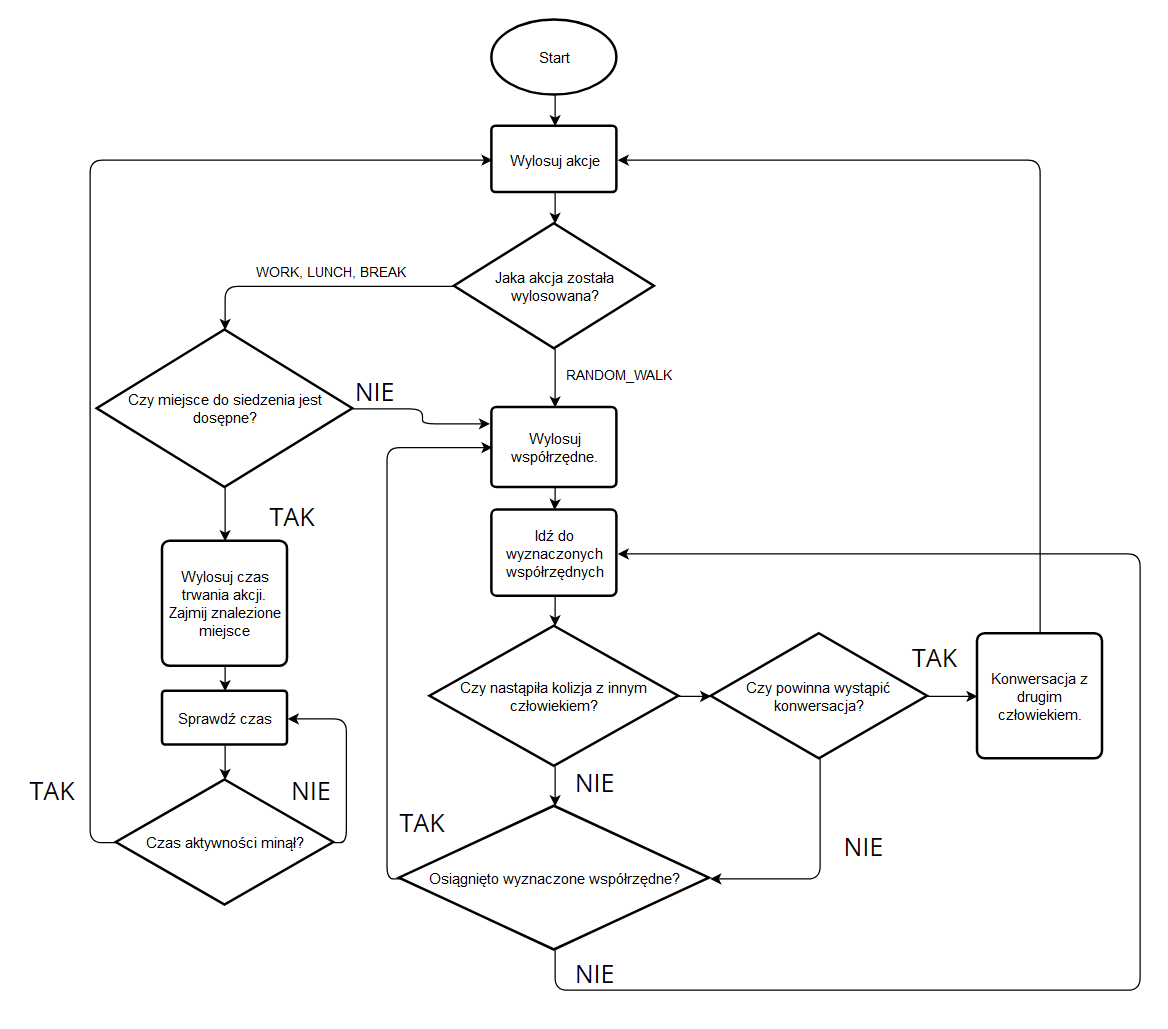
\includegraphics[width=\linewidth]{DiagramAlgorytmuZachowania.png}
	\caption{Sekwencyjny diagram algorytmu symulacji zachowań ludzkich}
	\label{diagramZachowanie}
\end{figure}


%Krótka wstawka kodu w linii tekstu jest możliwa, np.  \lstinline|int a;| (biblioteka \texttt{listings})% lub  \mintinline{C++}|int a;| (biblioteka \texttt{minted})
%. 
%Dłuższe fragmenty lepiej jest umieszczać jako rysunek, np. kod na rys \ref{fig:pseudokod:listings}% i rys. \ref{fig:pseudokod:minted}
%, a naprawdę długie fragmenty – w załączniku.


%\begin{figure}
%\centering
%\begin{lstlisting}
%class test : public basic
%{
%    public:
%      test (int a);
%      friend std::ostream operator<<(std::ostream & s, 
%                                     const test & t);
%    protected:
%      int _a;  
%     
%};
%\end{lstlisting}
%\caption{Pseudokod w \texttt{listings}.}
%\label{fig:pseudokod:listings}
%\end{figure}

%\begin{figure}
%\centering
%\begin{minted}[linenos,frame=lines]{c++}
%class test : public basic
%{
%    public:
%      test (int a);
%      friend std::ostream operator<<(std::ostream & s, 
%                                     const test & t);
%    protected:
%      int _a;  
%      
%};
%\end{minted}
%\caption{Pseudokod w \texttt{minted}.}
%\label{fig:pseudokod:minted}
%\end{figure}


